\documentclass[french]{article}
\usepackage[T1]{fontenc}
\usepackage[utf8]{inputenc}
\usepackage{lipsum}
\usepackage{lmodern}
\usepackage{geometry}
\usepackage{babel}
\usepackage{graphicx}
\usepackage{lastpage}
\usepackage{ragged2e}
\usepackage{enumitem}

\geometry{
 	a4paper,
 	total={210mm,297mm},
 	left=20mm,
 	right=20mm,
 	top=20mm,
 	bottom=20mm,
}

\usepackage{fancyhdr}
\pagestyle{fancy}
\setlist[enumerate,1]{leftmargin=2cm}

\lhead{Browne, Champion, Djomo,\\Hardy, Richoz, Rochat}
\chead{}
\rhead{07.03.2016}
\renewcommand{\headrulewidth}{0.4pt}
\renewcommand{\footrulewidth}{0.4pt}
	 
\begin{document}
	\centering
	\large{\textbf{PRO: cahier des charges}}
	
	\justify
	
	\section{Spécification}
		L'objectif global de ce projet est la réalisation d'une application de résolution de problèmes classiques des graphes dans le cadre du cours PRO. Elle sera réalisée en Qt afin de pouvoir être déployée sur les plateformes Linux, Mac OS et Windows mais ne sera que testée sur cette dernière.
		
		\subsection{Maquette (pas définitive)}
			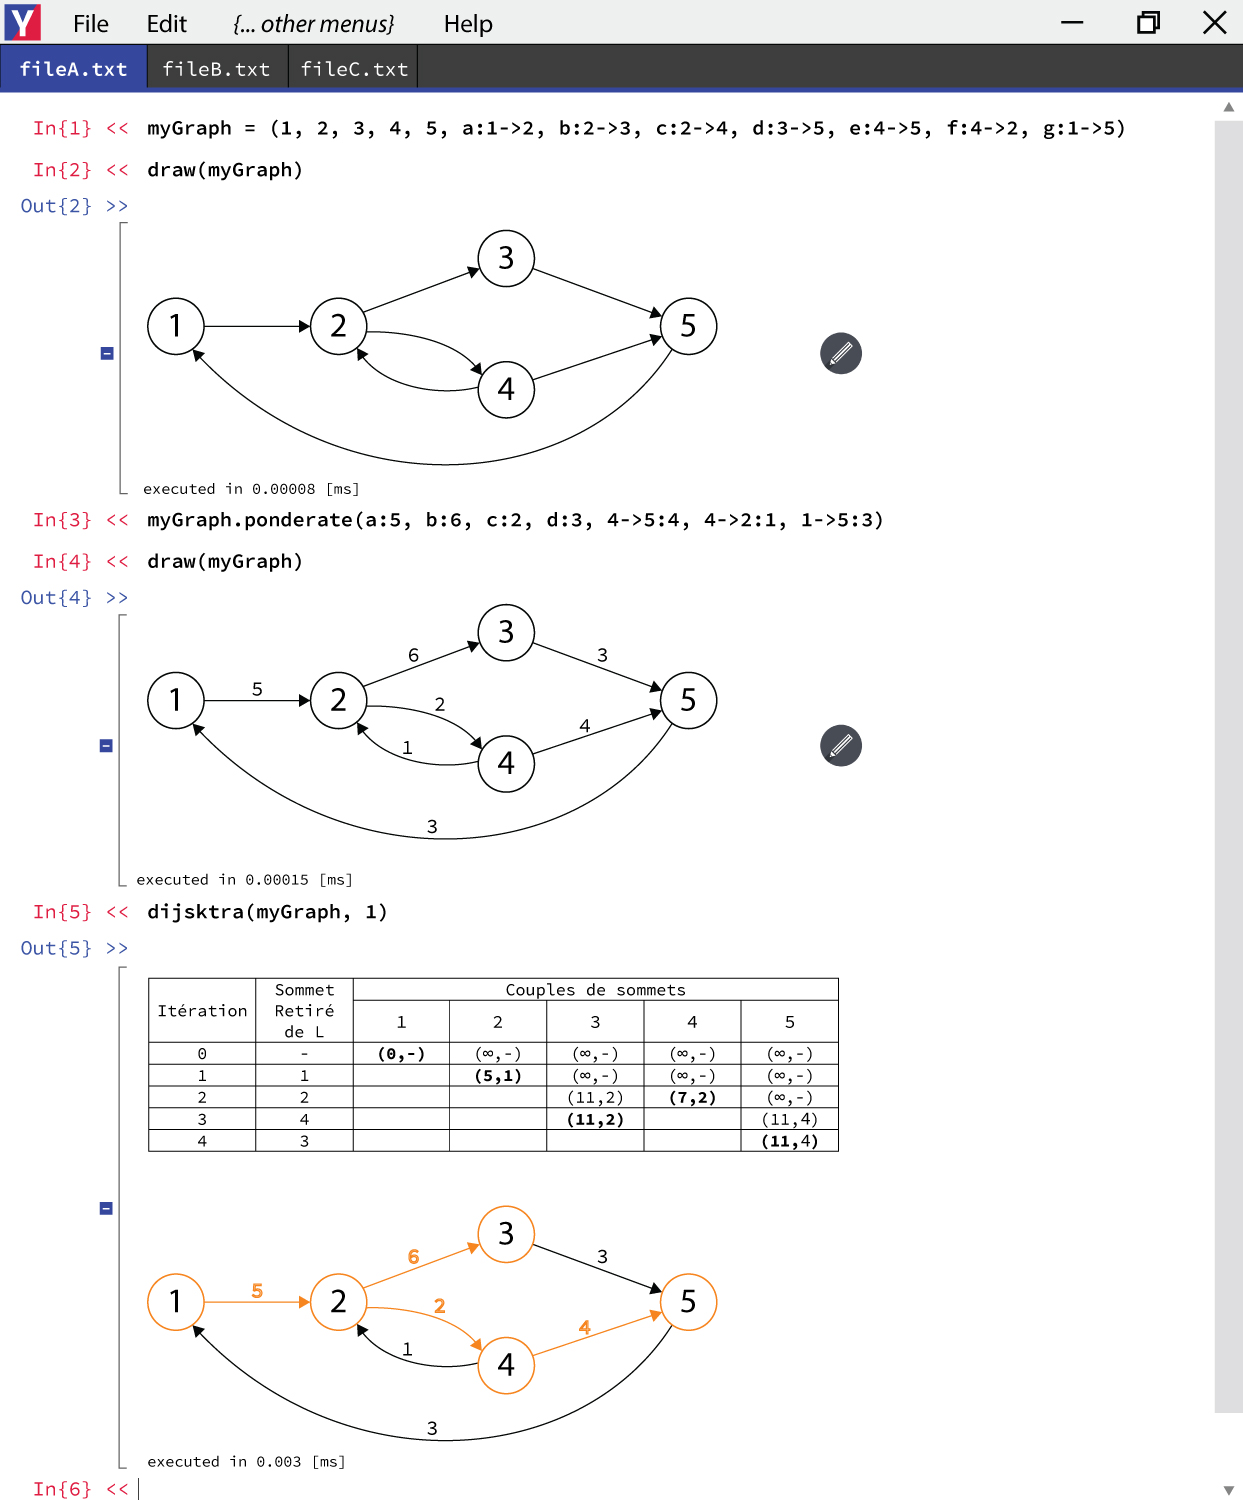
\includegraphics[width=0.9\textwidth]{maquette}
		
	\section{Fonctionalités}
		Les fonctionnalités suivantes devront être réalisées avant le 30 mai (semaine 14 du semestre). Les optionnelles seront à faire si le temps le permet, et les futures sont des améliorations de l'application non prévues dans le cadre du projet.
		\begin{enumerate}
			\item Saisie de graphes orientés ou non et pondérés ou non au moyen d'un langage spécifique.
			\begin{enumerate}
				\item Chargement d'un (grand) graphe depuis un fichier externe.
				\item (optionnelle) Génération aléatoire de graphe.
			\end{enumerate}
			
			\item Appliquer les algorithmes classiques aux graphes et afficher leurs résultats.
			\begin{enumerate}
				\item Les commandes peuvent être sauvées vers et chargées depuis un fichier texte.
				\item Plusieurs onglets peuvent être ouverts en parallèle.
				\item (optionnelle) Auto-complétion des fonctions et des variables pendant une saisie.
				\item (optionnelle) Historique des commandes avec les flèches HAUT et BAS.
				\item (future) Exécution/affichage étape par étape des algorithmes.
			\end{enumerate}
			
			\item Dessiner la représentation graphique d'un graphe défini précédemment.
			\begin{enumerate}
				\item Édition à la souris de la représentation graphique, reprise sur tous les dessins.
				\item Exportation des dessins au format SVG.
				\item (optionnelle) Exportation dans d'autres formats d'image.
				\item (future) Dessiner le graphe directement de manière optimale (avec le moins de chevauchement au niveau des arcs/arêtes).
			\end{enumerate}
			
			\item Un menu d'aide contenant les différentes entrées/fonctions possibles avec une documentation associée, ainsi qu'une option de recherche.
			\begin{enumerate}
				\item (future) Possibilité de lancer un algorithme via une fenêtre de dialogue.
			\end{enumerate}
		\end{enumerate}
		
		\subsection{Famille de graphe}
			Cette section précise les types de graphe gérés par l'application:
			\begin{itemize}
				\item Orienté / non-orienté
				\item Biparti / classique
				\item Sommet pondéré / non-pondéré
				\item Sommet avec capacité (min et max)
				\item Arête (arc) pondérée / non-pondérée
				\item Arête (arc) avec capacité (min et max)
			\end{itemize}
			
		\subsection{Algorithmes}
			Cette section précise les familles d'algorithme prévues dans l'application:
			\begin{itemize}
				\item Parcours du graphe (DFS, BFS)
				\item Tri topologique
				\item Détection de cycle
				\item Composante fortement connexe (Kosaraju, Tarjan) 
				\item Arbre recouvrant de poids min (Kruskal, Prim)
				\item Arborescence recouvrante de poids min (Chu-Liu)
				\item Arborescence recouvrante de section min/max (Prim orienté)
				\item Plus court chemin depuis un sommet (Acyclique, Bellman-Ford, Dijkstra)
				\item Flot de capacité fixée (ou max) (Ford-Fulkerson)
				\item Flot de capacité fixée (ou max) de poids min (Busacker-Gowen)
				\item (optionnel) Problème de transbordement
				\item (optionnel) Plus courts chemins depuis tous les sommets (Floyd-Warshall, Johnson)
				\item (futur) Couplage max (de poids min)
				\item (futur) Postier chinois
			\end{itemize}
			NB: les noms entre parenthèses sont des exemples d'algorithmes pouvant être implémentés.
		
	\section{Planification}
		\subsection{Liste des tâches}
			(listes des tâches avec leur durée estimée et leur dépendance)
		\subsection{Graphe potientiels-tâches}
			(éventuellement)
		\subsection{Diagramme de Gantt}
			(avec prise en compte des retards)
			
\end{document}
